\documentclass[class=article, crop=false]{standalone}
\usepackage{default}

\begin{document}
Consideremos una parcela de aire de volumen $dV=Adz$, como el de la figura \ref{dV}.
\begin{figure}
   \centering
   \vspace{5mm}
   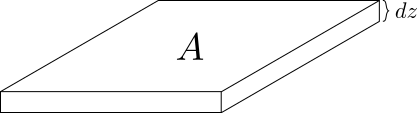
\includegraphics[width=0.5\linewidth]{dV.png}
   \caption{Parcela de aire muy pequeña, de volumen $Adz$.}
   \label{dV}
\end{figure}

La masa de aire dentro de esta parcela es $dM = \rho_A dV$, con $\rho_A$ la densidad del aire. Ahora, como la parcela es bien delgada (con cambio de altura minimo) podemos asumir que la ecuación de estado $P = \rho_A R_d T_v$ se cumple. Con esto último en cuenta, despejamos la densidad de la ecuación de estado y la expresión para la masa nos queda
\begin{equation}
    dM = \frac{P}{R_dT_V}A\,dz \label{dM}
\end{equation}
Dentro de esta parcela, la cantidad de masa de (vapor de) agua será simplemente $dM_W = qdM$, con $q$ la humedad específica dentro de la parcela. Ahora, ¿Que volumen ocuparía toda esa masa de vapor de agua se condensase?. Este volumen sería equivalente a $dM_W/\rho_W$, con $\rho_W$ la densidad del agua (en estado liquido), lo que es equivalente a  
\begin{align*}
    dV_W &= \frac{dM_W}{\rho_W}\\
         &= \frac{qdM}{\rho_W}\\
    dV_W &= \frac{qP}{R_dT_V \rho_W}A\,dz \label{dMW}
\end{align*}
Consideremos lo siguiente ahora. El volumen de agua condensada lo pondremos en una columna de area transversal $A$, como en la figura \ref{dVW}
\begin{figure}
    \centering
    \vspace{3mm}
    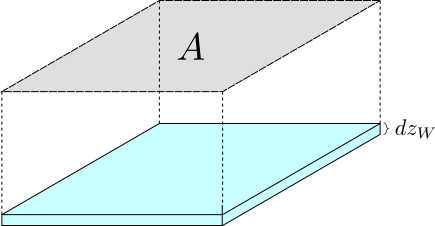
\includegraphics[width=0.52\linewidth]{dVW.png}
    \caption{Volumen de agua condensada en una columna de area transversal $A$.}
    \label{dVW}
\end{figure}
Acorde a la figura, nombraremos $dz_W$ a la altura de la columna de agua. Notemos que $dz_W = dV_W/A$. Con esto en cuenta llegamos a la siguiente expresión
\begin{equation}
   dz_W = \frac{qP}{R_dT_V \rho_W}\,dz \label{dzW} 
\end{equation}
En resumen, la ecuación \eqref{dzW} nos dice que tendremos un nivel de precipitación (por unidad de área, y en unidades de longitud) $dz_W$, para una columna de aire de altura $dz$. Ahora, para obtener el nivel de precipitación de una columna aire de altura $z_1$ (con $z_1 \gg dz$) con su base a nivel del mar, hay que integrar. Entoces, la expreción para el nivel de precipitación queda
\begin{equation}
    z_W = \int_0^{z_1} \frac{q(z)P(z)}{R_d T_v \rho_W} dz \label{zW}
\end{equation}
Notemos que ahora sí consideramos la dependencia en $z$ de $q$ y $P$. Recordemos también que estas equivalen a
\begin{equation}
    q(z) = q_0 e^{-z/H_v} \label{qz}
\end{equation}
\begin{equation}
    P(z) = P_0 e^{-z/H} \label{Pz}
\end{equation}
con $q_0 = 10\,$[g/Kg], $H_v = 3\,$Km, $P_0 = 1013\,$hPa y $H = 8\,$Km.\\ 

Remplazamos \eqref{qz} y \eqref{Pz} en \eqref{zW} y nos queda
\begin{equation}
    z_W(z_1) = \int_0^{z_1} \frac{q_0 P_0}{R_d T_v \rho_W} e^{-z/\bar{H}} dz \label{zW2}
,\end{equation}
con $\bar{H} = \frac{H_v H}{H_v + H} = \frac{24}{11}\,$Km. Para integrar \eqref{zW2} de forma sencilla asumiremos que el ni $R_d, T_v$ ni $\rho_W$ dependen de $z$. Entoces, el nivel de precipitación resulta
\begin{align*}
    z_W(z_1) &= \frac{q_0 P_0}{R_d T_v \rho_W} \int_0^{z_1}  e^{-z/\bar{H}} dz \label{zW2}\\
        &= - \frac{q_0 P_0\bar{H}}{R_d T_v \rho_W}  e^{-z/\bar{H}}\Bigg|_{0}^{z_1}\\
        &= - \frac{q_0 P_0\bar{H}}{R_d T_v \rho_W}(e^{-z_1/\bar{H}} - 1)
\end{align*}
Recordemos que de \eqref{Pz} tenemos que $H = \frac{R_d T_v}{g}$, por lo que podemos simplificar lo anterior.
\begin{align*}
    z_W(z_1) &= \frac{q_0 P_0 \bar{H}}{\rho_W g H} (1 - e^{-z_1/\bar{H}})\\
             &= \frac{q_0 P_0}{\rho_W g H} \frac{H_v H}{H_v + H} (1 - e^{-z_1/\bar{H}})
\end{align*}
Finalmente, queda
\begin{equation}
    z_W(z_1) = \frac{q_0 P_0}{\rho_W g} \frac{H_v}{H_v + H} (1- e^{-z_1/\bar{H}})
\end{equation}

\end{document}
